% !Mode:: "TeX::UTF-8"
\documentclass[a1,portrait]{sciposter}

%% uzitocne package
\usepackage{multicol}
\usepackage{color}
\usepackage{graphicx}
\usepackage{amsmath}

%% znaky s diakritikou
\usepackage[utf8]{inputenc}
\usepackage[T1]{fontenc}
% \usepackage[slovak]{babel} % slovenske delenie slov

%% definicia farieb
\definecolor{mainCol}{rgb}{0.91,0.82,0.74} % farba pozadia posteru
\definecolor{sectionCol}{rgb}{0,0,0} % farba nadpisu
\definecolor{textCol}{rgb}{0.2,0,0} % farba hlavneho textu
\definecolor{BoxCol}{rgb}{1,1,0.8} % farba boxu okolo nadpisov

\def\mysection#1{
{\color{sectionCol}\section*{\sc\bfseries #1}}}

\let\oldfootnoterule\footnoterule

\addtolength{\skip\footins}{0pt}

\def\footnoterule{\vskip-5pt\oldfootnoterule \vskip20pt\relax}

\begin{document}
\setlength{\logowidth}{20cm}
\setlength{\titlewidth}{\textwidth}
\addtolength{\titlewidth}{-\logowidth}
%\userightlogotrue
\rightlogo[1]{color_uniba}
\useleftlogotrue
\leftlogo[1]{color_fmph}

\color{textCol}

\title{Wearable EEG-Based Brain-Computer
Game Controlling Interface}
\author{Viktor Seč$^1$\footnote{hey@viktorsec.com}\\
        Supervisor: Barbora Cimrová$^1$ $^2$}
\institute{%
$^1$ Department of Applied Informatics,
FMPH UK, Mlynská Dolina, 842~48~Bratislava
$^2$ Laboratory of Cognitive Neuroscience, UNPF SAV, Sienkiewiczova 1, 813 71 Bratislava
}

\maketitle

\begin{multicols*}{3}

\mysection{Introduction}

EEG-based Brain Computer Interface (BCI) employing motor imagery enables direct communication between the user's brain and a computer \cite{schlogl2005characterization}. The user images moving his body, causing short moments of \emph{mu} (8 – 12 \emph{Hz}) and sensorimotor (12 – 15 \emph{Hz}) rhythm desynchronizations in the sensorimotor cortex \cite{mcfarland2000mu} of the brain. These are acquired by an EEG device and can be detected in the output signal by a computer program -- when done in real time, this task is called an online classification.

We've built an end-to-end BCI solution utilising a wearable headset.

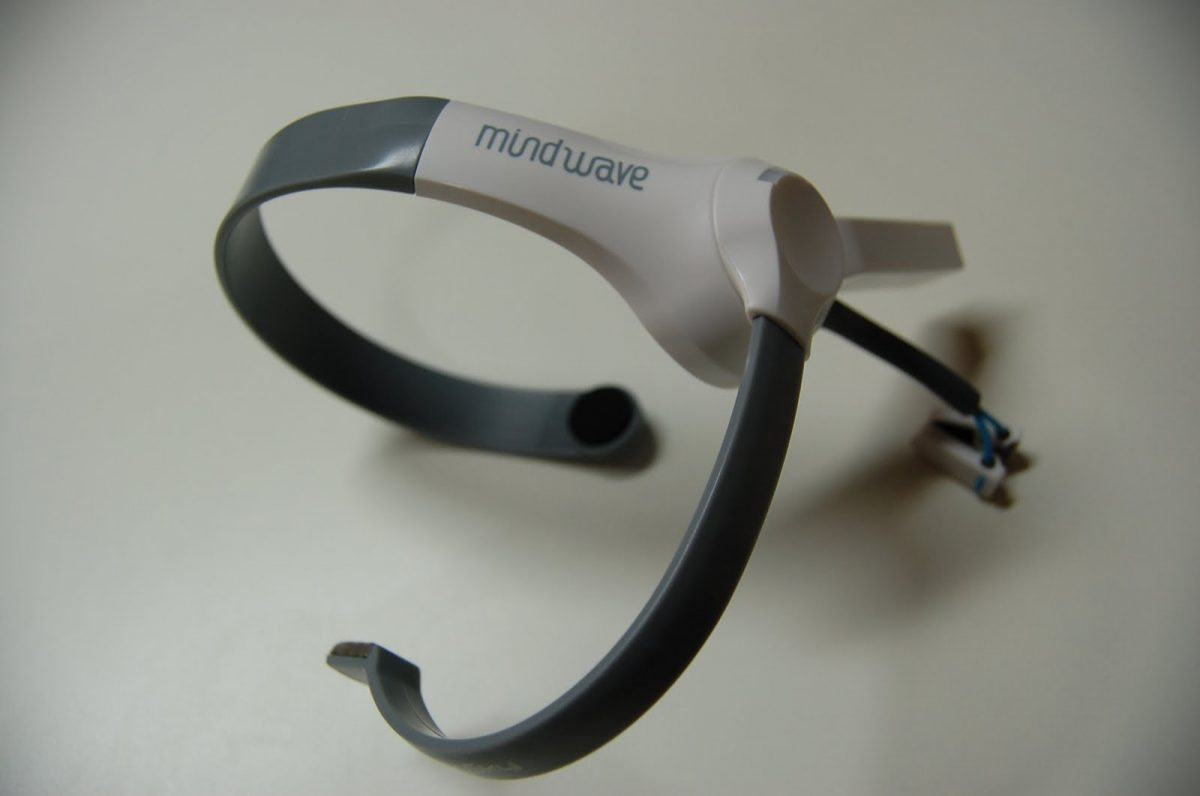
\includegraphics[width=\columnwidth]{mindwave}
\caption{NeuroSky MindWave EEG headset} 

\mysection{Methods}

We record the signals with \emph{NeuroSky MindWave}, an economical EEG headset equipped with on-board bluetooth connectivity. This device is reasonably priced, compact and gives user high freedom of movement. However it also bears only one electrode, which poses a challenge as we are unable to easily topographically distinguish the source of detected neural activity. We put this electrode on C3 position of the 10-20 system.

We acquire the signal using OpenVIBE server, which sends it to OpenVIBE Designer \cite{renard2010openvibe}. We've set up an online classifier in OpenVIBE to classify received signals.

We've recorded sample training data in two conditions -- state of rest and hand motor imagery. We used these data offline to teach a classifier.

The signal was first processed with temporal band pass filter selecting frequencies between 1 and 20 \emph{Hz}. Next we cut it into epochs of 1 second every \( \frac{1}{16} \)th of a second. We feed the average signal of every epoch into feature aggregator which extracts a feature vector. The feature vectors of both conditions are put into classifier trainer which computes a classifier.

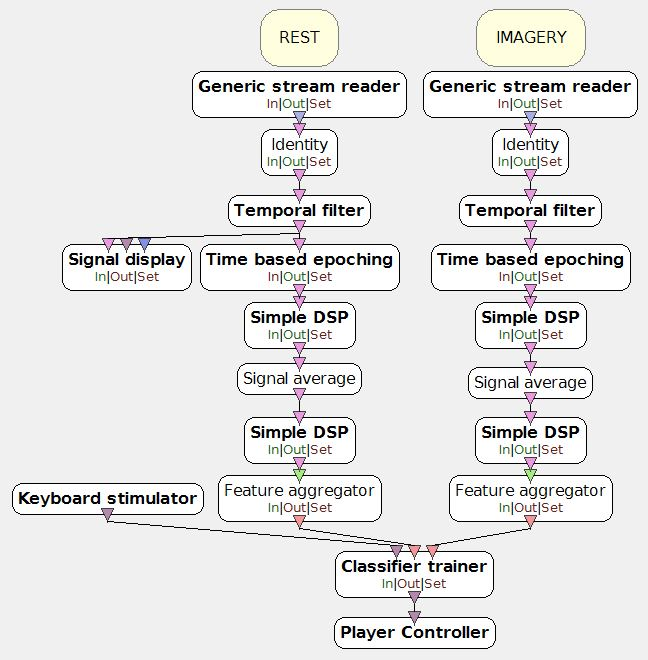
\includegraphics[width=\columnwidth]{training}
\caption{Training scenario in OpenVibe}

We are now able to aquire new signals and classify it online (in real time) with our classifier, effectively creating a brain switch. This switch produces one dimensional control output signal.

\mysection{Results}

The classifier accuracy is around 57\%. Trying to improve it, we've replaced the Mindwave's original electrodes for better ones. This considerably raised the signal quality, however performance of our classifier remains fairly low.

We use the online classifier to control a simple game, which we are building in the \emph{Unity} game engine.

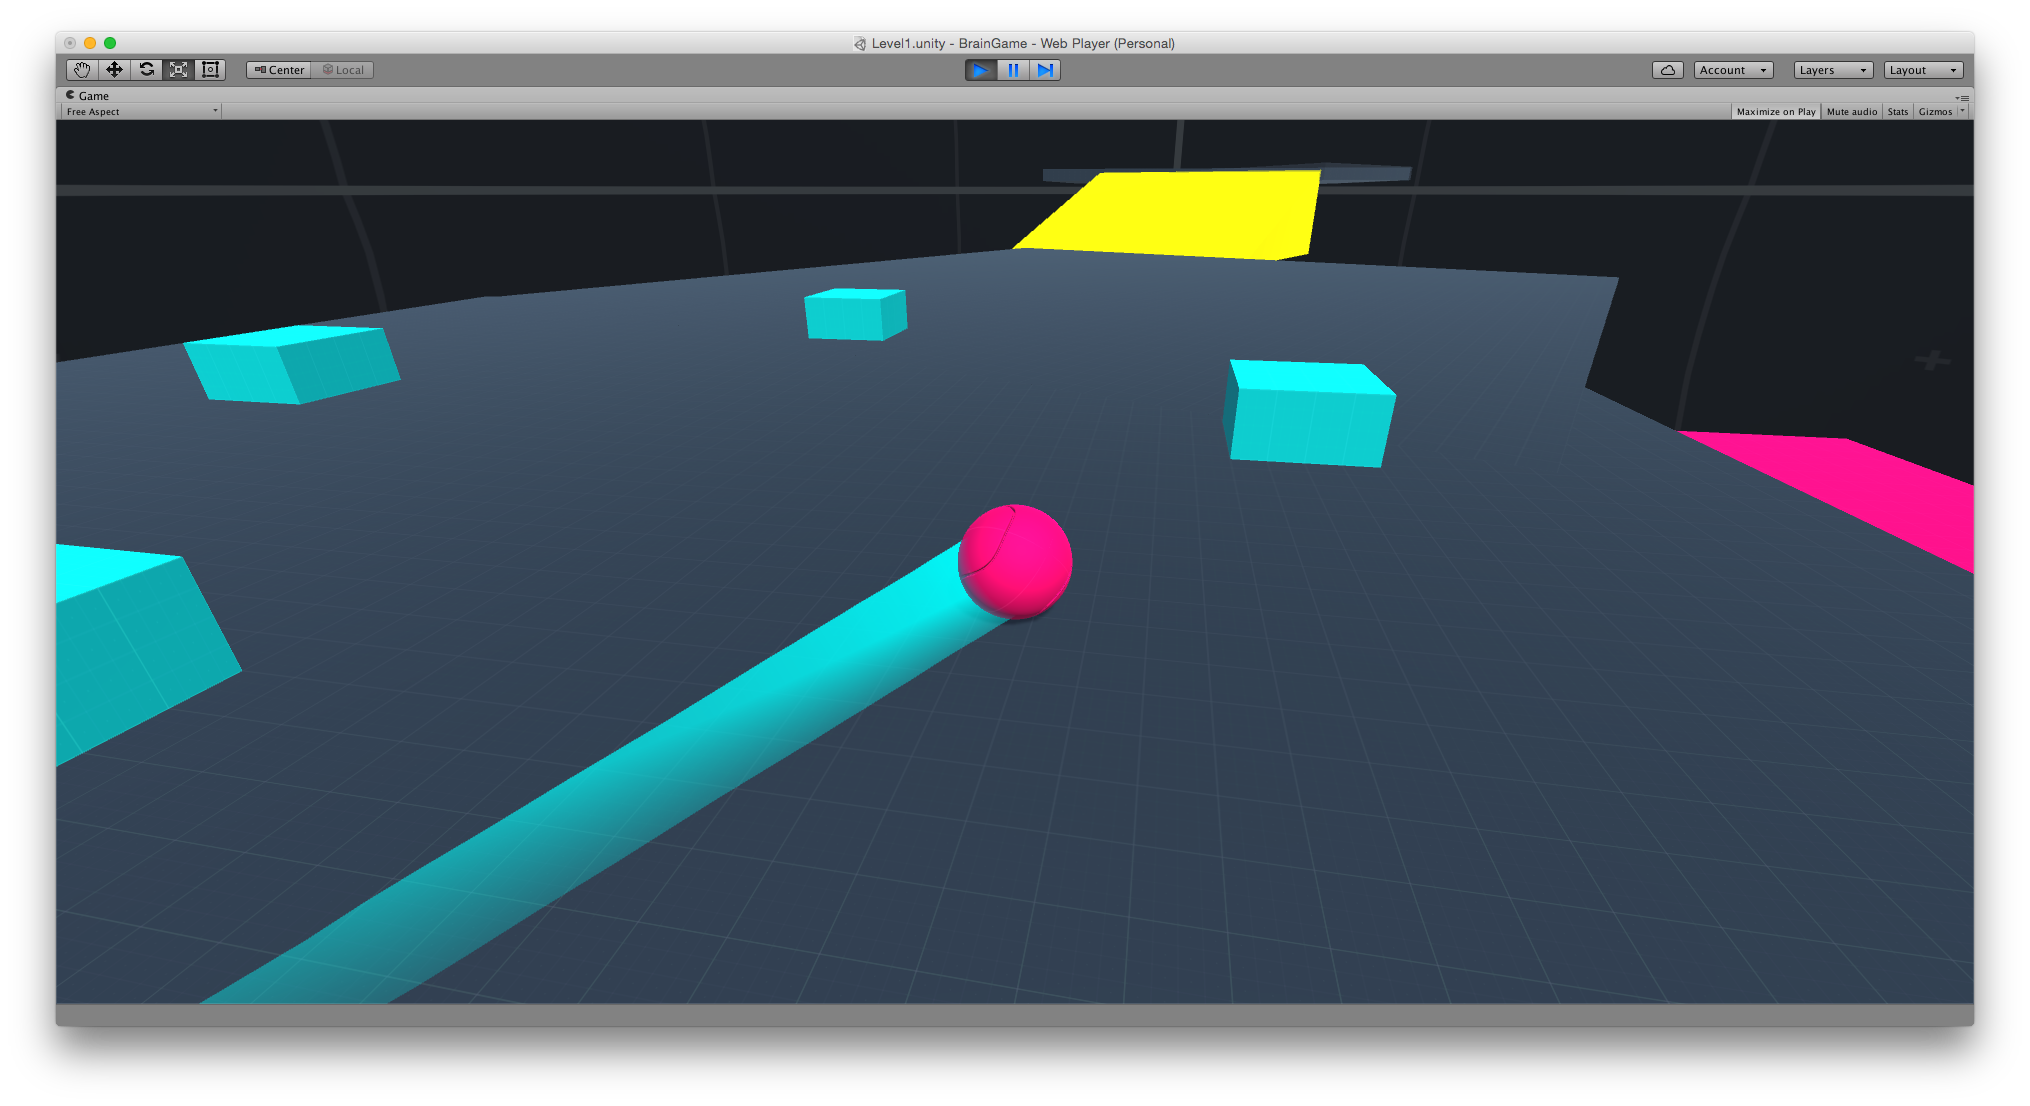
\includegraphics[width=\columnwidth]{game}
\caption{Proposed game implemented in Unity} 

\mysection{Discussion}
We attribute the performance deficiency to using only one EEG chanel and recommend utilizing multiple electrodes in simple motor imagery BCIs.

\mysection{Attachments}
All code and project files are available at http://dx.doi.org/10.5281/zenodo.56235

\mysection{Acknowledgements}

I would like to express my thanks to Barbora Cimrová for supervising, Štefan Bendžala for hardware help and Dominik Lukáč for participating in experiments.

\begin{small}
%% zoznam literatury
\bibliographystyle{apalike}{\small}
\bibliography{references}
\end{small}

\end{multicols*}
\end{document}

